\documentclass[a4paper, 10pt]{article}
\usepackage[utf8]{inputenc}
\usepackage{verbatim}
\usepackage{listings}
\usepackage{graphicx}
\usepackage[english]{babel}
\usepackage{a4wide}
\usepackage{color}
\usepackage{amsmath}
\usepackage{float}
\usepackage{amssymb}
\usepackage[dvips]{epsfig}
\usepackage[toc,page]{appendix}
\usepackage[T1]{fontenc}
\usepackage{cite} % [2,3,4] --> [2--4]
\usepackage{shadow}
\usepackage{hyperref}
\usepackage{titling}
\usepackage{marvosym }
\usepackage{subcaption}
\usepackage[noabbrev]{cleveref}
\usepackage{cite}
\usepackage[most]{tcolorbox}


\setlength{\droptitle}{-10em}   % This is your set screw

\setcounter{tocdepth}{2}

\lstset{language=c++}
\lstset{alsolanguage=[90]Fortran}
\lstset{alsolanguage=Python}
\lstset{basicstyle=\small}
\lstset{backgroundcolor=\color{white}}
\lstset{frame=single}
\lstset{stringstyle=\ttfamily}
\lstset{keywordstyle=\color{red}\bfseries}
\lstset{commentstyle=\itshape\color{blue}}
\lstset{showspaces=false}
\lstset{showstringspaces=false}
\lstset{showtabs=false}
\lstset{breaklines}
\title{AST1100 rapport}
\author{Daniel Heinesen, daniehei}
\begin{document}
\maketitle

\begin{abstract}
In this articles I am interested simulating a complete interplanetary space voyage. I am going to look at the construction of an easy rocket engine, how we can simulate an entire solar system, how to transverse the large empty space between it's planets and finally how to land on one of the planets. On the way we are going to try to orient, and try to analyze the atmosphere to the target planet. Last we are going to put these simulation to the test and send a satellite to this planet, and hopefully manage to land safely.
\end{abstract} 

\paragraph*{Constants and Variables}

\begin{center}
\begin{tabular}{l  c}
$k$ & Boltzmann's constant.\\
$F_b$ & Force from \textit{one} box. \\
$n_b$ & Number of boxes.\\
$m_l$ & Mass of the satellite. \\
$m_f$ & Mass of the fuel.\\
$m_e$ & Mass of the particles escaping per second per box. \\
$m_{f0}$ & Mass of fuel when launching. \\
\end{tabular}
\end{center}



\tableofcontents

\section{Introduction}

In this articles we shall look at many of the aspects of sending and landing a spacecraft on out neighbor planet Isskji. \\

We are first going to look at the engine, approximating it by a simple "particle in a box" model, and seeing what kind of force we can expect. We will then you Newton's law of gravity for N-bodies, and simulate our solar system. We also what to see if Isskji is in the habitable zone, and if the trip is worth taking. Having a knowledge about how out solar system will look in the future, we can begin to plan out trip, doing some calculations using Hohmann transfers and seeing if this can get us to Isskji. With list of maneuvers we need to get to our destination, we can look at the fuel usage, and deriving a rocket equation specific for our engine. \\

Under way to Isskji, the spacecraft need a way of knowing where it is. By getting data about the distance to the other planets, the spectrum of two distant star and pictures of the starscape, it will be able, though gradient descent, Doppler shift and least square comparisons to find all the information it needs to orient it self.\\

Finally in orbit around Isskji, we need to make a model of the atmosphere to see how big a parachute the lander will have to have to safely land on the planet. We also have to scout the planet, finding a good place to land, and calculate the trajectory needed to get us to our desired landing point.

We want to acknowledge some of the other space agencies who has been researching the same problems. A special thanks to Gunnar Lange, Fredrik Mellbye, Erlend Liam og Aram Salihi for make this possible.

\section{Theory and Methods}

\subsection{The Engine}

To simulate the engine we are going to approximate the complex going-ons in a rocket engine by a box of particles with a hole in the floor. The particles only interact with the walls, thus making them an ideal gas. As some particles leave the hole in the floor, momentum are lost. By pumping in more gas, keeping the pressure constant, momentum is conserved. This means that for every particle escaping, some momentum is lost straight downward, and the box gets a momentum equal to that of the particle, but in the opposite direction. The result is that the engine moves upwards. Since $H_2$ is one of the most used fuels, out gas will consist of $H_2$ molecules.\\

The box is a cube, with sides $L = 10^{-6}m$. The box is simulated with the orgin at the center, this gives us completely symmetry, making the code easier. The particles are placed with a uniform distribution 

\begin{align}
p(x) = \frac{1}{b-a}\Theta(x-b)\Theta(a-x)
\end{align}

in the box, with a velocity, the components distributed with the \textit{M axwell-Boltzmann distribution}

\begin{align}
P(v_i) = \sqrt{\left( \frac{m}{2 \pi k T} \right)} e^{-\frac{m v_i}{2kT}}
\end{align}

This is a Gaussian distribution with $\sigma = \sqrt{ \frac{kT}{m}}$
and $\mu = 0$.\\

To check if the simulation gives us a realistic gas simulation, we check if the analytical and numerical kinetic energy and pressure are the same. We find the numerical pressure by first look at the force on one wall:
\begin{align}
F_i = \frac{dp}{dt} \approx \frac{\Delta p}{\Delta t} = \frac{2p_i}{\Delta t}
\end{align}
This gives us the pressure:
\begin{align}
P = \frac{F}{A} = \frac{\frac{2p_i}{\Delta t}}{A} = \frac{2p_i}{\Delta t L^{2}}
\end{align}

The analytical expression for the pressure of an ideal gas is:

\begin{align}
P = nkT
\end{align}


The kinetic energy is given by:

\begin{align}
E_k = \frac{1}{2n}m_{h2}\sum\limits_{i=1}^{n}(v_x^{2} + v_y^{2} + v_z^{2})
\end{align}

numerically and
\begin{align}
 E_k = \frac{3}{2}kT
\end{align}

analytically. \\

A hole with the size $H =\frac{L}{2}$ is opened in floor, and the number of particle escaping is counted, that the momentum gained by box is calculated.\\

An important choice is what to do when a particle escape. Since we want the pressure to be constant over time, we have to find a method of placing the escaped particles back in the box. One way is to place the particle back in the box with a random position and velocity. This sounds to be the easy and correct way to do this, but one thing we noticed was that both the pressure and kinetic energy has a tendency to decrease over time. We speculate that this is because the particle with higher velocities has the greatest chance of hitting the floor and being placed back in the box with a new random velocity, thereby skewing the velocity distribution towards lower velocities. The way we went for was to just let the particles bounce back just as if they hit the other walls. This guaranties that the kinetic energy and pressure stays the same. 

\subsection{A simple launch}

Before we send the spacecraft on the full journey, we want to see what it is capable of with a small launch to reach escape velocity. Escape velocity is given by 

\begin{align}\label{eq:escape}
v = \sqrt{\frac{2GM}{r}}
\end{align}

As we will see in the results, one box is far from enough to get us anywhere. To find the amount of boxes we need to give us sufficient force, we are going to see how many boxes we need to get escape within a somewhat randomly picked time of 10 min.

\begin{align}
v(t) = \frac{F}{m} t = \frac{F_{per box}n_{boxes}}{m_{launcher}} t
\end{align}

\begin{align}\label{eq:boxes}
n_{boxes} = \frac{v m}{F t}
\end{align}

We are now going to assume that the fuel does not contribute to the mass of the spacecraft, and see how much fuel is needed to get to escape velocity. Since this is an unrealistic assumption, we have to have an analytical expression for the needed fuel. In the appendices in section \ref{sec:Fuel} this is shown to be:

\begin{align}\label{eq:Fuel}
m_{f0} = m_l(e^{\frac{\Delta v m_e}{F_b}} - 1)
\end{align}

We are going to check if this equation gives us the correct amount of fuel.



\section{Results and Discussion}

\subsection{The Engine}

The fist result is the pressure and kinetic energy inside of the box:
\begin{tcolorbox}
Numerical Pressure:  13756.1188494 \\
Analytical Pressure:  13800.0 \\
Analytical energy:  2.07e-19 \\
Numerical energy:  2.06623799518e-19 
\end{tcolorbox}

As we can see, the numerical and analytical results have relative errors within a factor of $10^{-4}$, meaning that out simulation are quite accurate.

The data from the engine was as follows:

\begin{tcolorbox}
Force:  1.72650965887e-09 \\
Number of particles colliding with floor:  257317 \\
Number of particles escaped:  64252 \\
Number of particles escaped per sec:  6.4252e+13 \\
Mass lost per sec:  2.120316e-13
\end{tcolorbox}

We can see that the force exerted by a single box is minuscule, and a lot of boxes are needed to lift the spacecraft of the ground. \\

The data above are from one specific simulation, and will vary enough to make results in later parts of this article a bit different. We will therefor use the data given here for all subsequent situations where they are needed.

\subsection{A simple launch}

Using equation \ref{eq:escape} we see that $v_{escape} \approx 16596.9 m/s$. And from \ref{eq:boxes} we get that the amount of boxes we need are $n = 1.76 \cdot 10^{13}$. \\

The plot we get from launching the spacecraft without fuel loss:


\begin{figure}[H]
\begin{center}
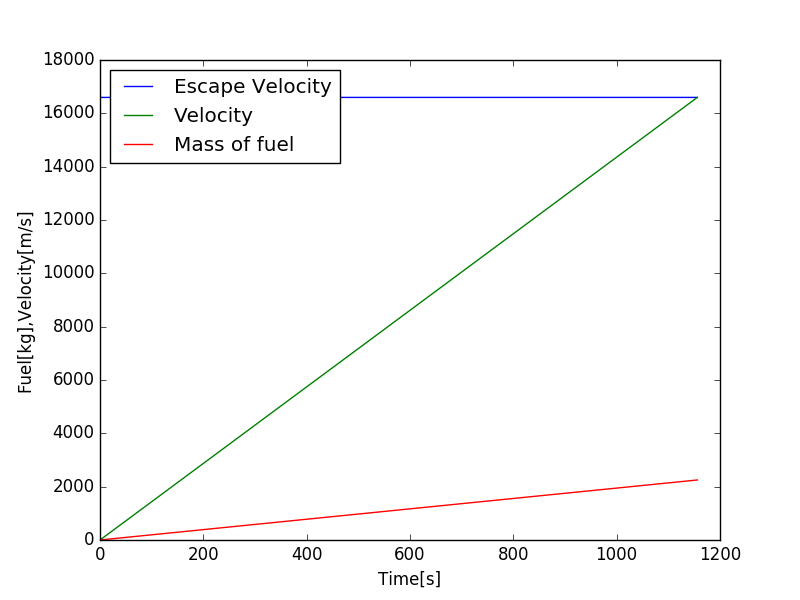
\includegraphics[width = 70mm]{part1launchConstMass.png}
\caption{Shows the mass of fuel increasing has the spacecraft accelerates. The craft end up using right under 2000 kg of fuel.}
\end{center}
\end{figure}

The plot of the launch with fuel loss shows how the spacecraft loses fuel as it ascends. The initial fuel was given by equation \ref{eq:Fuel} as $2250.966 kg$.


\begin{figure}[H]
\begin{center}
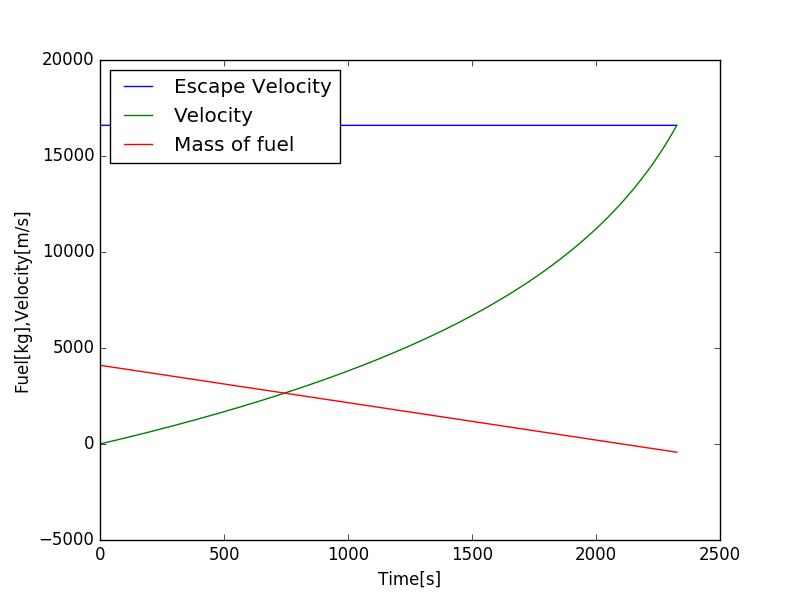
\includegraphics[width = 70mm]{part1launchVarMass.png}
\caption{Shows the mass of fuel slowly going to zeros as the spacecraft reaches escape velocity.}
\end{center}
\end{figure}

We can see from the plot over that as the spacecraft reaches escape velocity, the mass of the fuel is more or less zero. This indicates that out expression for fuel gives the correct amount of fuel.

\section{Appendix A: Symbols and Parameters} 
\begin{itemize}
\item $F_b$: Force from \textit{one} box.
\item $n_b$: Number of boxes.
\item $m_l$: Mass of the satellite.
\item $m_f$: Mass of the fuel.
\item $m_e$: Mass of the particles escaping per second per box.
\item $m_{f0}$: Mass of fuel when launching.
\end{itemize}

\section{Appendix B: Fuel Equation}\label{sec:Fuel}

To find an analytical expression for the fuel use, we are going to derive the rocket equation using the parameters we get from out engine. We are going to start with Newton's 2. law to find the acceleration for our system:

\begin{equation}
a = \frac{F}{m} = \frac{F_b n_b}{m_f(t) + m_l} 
\end{equation}

Since the system are losing mass:

\begin{equation}
a = \frac{F_b n_b}{(m_{f0} - n_b m_e t) + m_l} = \frac{F_b n_b}{(m_{f0} - \Delta m t) + m_l}
\end{equation} 

Where $m_{f0}$ is the initial mass of the fuel, and $\Delta m$ is the mass loss per second. We separate the variables and solve the differential equation:

\begin{equation}
v(t) = \int \frac{F_b n_b}{(m_{f0} - \Delta m t) + m_l} dt
= K - \frac{F_b}{m_e} \ln(m_{tot} - \Delta m t) 
\end{equation}

Where $m_{tot} = m_l + m_{f0}$. Using the boundary expression we find

\begin{equation}
K = v_0 + \frac{F_b}{m_e} \ln (m_{tot})
\end{equation}

This gives us the rocket equation for our satellite: 

\begin{equation}
v(t) =v_0 + \frac{F_b}{m_e} \ln \left(\frac{m_{tot}}{m_{tot} - \Delta m t} \right)
\end{equation}

We can see that $\frac{F_b}{m_e}$ has the dimension of velocity. This expression corresponds to the velocity of particles escaping (exhaust velocity). If we call this $v_e$ we have the original rocket equation. We want to have use all the fuel when the desired $\Delta v$ i reached. The only mass left then is the mass of the satellite, so $m_{tot} - \Delta m t = m_l$. From this we can find the equation for fuel needed:

\begin{equation}
m_{f0} = m_l(e^{\frac{\Delta v m_e}{F_b}} - 1)
\end{equation}






\end{document}